\section{Hardware}
The motivation of this project was a scalable system and the design of the HDL is intended to be built such that it can be implemented on any FPGA hardware with the relevant ports. For the purposes of testing in this project three DE0 FPGAs will be used (shown in Figure \ref{fig:de0}).


The Terasic DE0 board contains an Altera CYCLONE III FPGA with 15,408 logic elements and 512kb of memory. This chip is capable of hosting around 9 pixels from the original algorithm within around 10 000 logic elements. This board has a relatively large number of general purpose input/output ports with 2 40-pin connectors on the side of the board. It also has a 5-pin RS232 specification UART which may be used for host computer to device simulation. 

In order to  ensure that the design of the system is scalable to other architectures and interfaces, the UART controller can be logically partitioned and replaced in other applications as will be discussed in the HDL design.  First estimates of the number of interconnect ports needed are around 40 pins minimum with the scaling as the design parameters change. As these FPGA development boards are available freely within the department they will be used for the prototype system design. It is important to note however, that this should not impact the design in such a way that stops the design from being easily moved to other boards when necessary. A secondary benefit of this board is the large number of user input/output ports such as 4 7-segment displays which can be used for debugging and progress checking.  This board was freely available within the department and therefore made a good low cost prototyping unit, however these boards can be bought at a retail price of \$120. 


\begin{figure}[h!]
  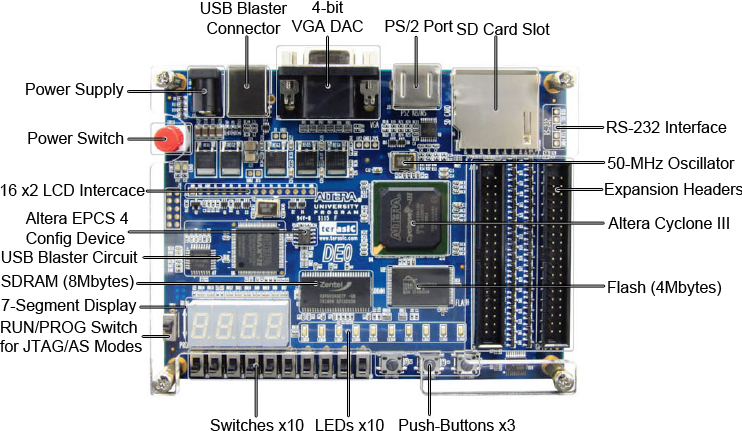
\includegraphics[width=\textwidth]{./figs/de0.png}
  \caption{Terasic DE0 FPGA Board}
  \label{fig:de0}
\end{figure}


An important decision to be made in the design of the hardware was whether to use a common clock across all the devices, or to use separate clocking. The advantage of the single clock is that the processors can work in lock-step reducing communication delays and simplifying the interconnect protocol. However, a common clock places other limitations on the design. The common clock design limits the clock frequency of all the devices to the speed at which the inter-FPGA communication can happen, this may lower the theoretical maximum clock speed, however the design already runs at a relatively low clock speed and the intentional is to overcome this limitation with parallelisation. The common clock will need to be considered in the testing stage, as identifying the clock speed where correct operation is primarily done through trial and error with a trade-off between bit-error rates and speed. The ring network design of this system favours the common clock approach as all communication is exclusively done with nearest neighbours, limiting the length of the inter-FPGA communications. 

\subsubsection{Inter-Device Communication Hardware}
All inter-FPGA communications will be done using the 40-pin GPIO connectors that were discussed earlier. The communication is done exclusively in a ring, which lends itself to a dual connector geometry. For each device the second GPIO connector will be linked to the first GPIO connector of the next device, with the final device looping back to the first connector of the first device. This is better than all-to-all communication, as that would scale extremely badly with number of devices as well as using far more ports. This takes care of the communication, however it is also necessary to have a shared global clock. This is achieved by separating one of the wires from the ribbon cable that connects the GPIO and connecting it together. This design is shown in figure \ref{fig:interfpga}, and is shown implemented on the board in the implementation section, figure \ref{fig:cluster}. The practical applications of this is also considered in the implementation section where the speed of the connection is analysed. 

\begin{figure}[h!]
  \includegraphics[width=\textwidth]{./figs/interfpga.pdf}
  \caption{Inter-FPGA Communication Hardware Setup}
  \label{fig:interfpga}
\end{figure}

\subsubsection{UART Hardware}
The UART interface on the board is theoretically designed to interface with any other RS232 standard UART controller, and the data streaming protocol will be covered in the Device Software section. For the purposes of interfacing with a host computer a USB to UART cable has been bought. Capable of up to 1~Mbaud the FTDI USB-RS232, this cable allows communication between the host software and device software using a virtual COM port for which there are multiple Application Programming Interfaces (APIs) available. The 1~MBaud limit allows up to 921,600 bits per second to be transmitted, when this is considered in the scope of the streaming project where each pixel has  a 2 bit data sample taken in the order of seconds and a DE0 FPGA can fit around 10 Pixels per device, the data rates this interface is capable of far exceed the rates needed. Only when devices with hundreds of pixels are present or extremely large arrays of devices are used will this present a problem. On the DE0 board a level shifter is present, this turns the 3.3v device signals into the $\pm$13v standard that RS232 uses.
